\hypertarget{energie-en-vermogen}{%
\chapter{Energie en Vermogen}\label{energie-en-vermogen}}

\lettrine{H}et gebruik van energie is een economische handeling die door economen nauwkeurig onderzocht moet worden, aangezien het vergelijkbaar is met handel, kapitaalaccumulatie en geld als een methode om de kwaliteit en kwantiteit van onze tijd op aarde te verhogen. Hoewel economische leerboeken, zowel de mainstream als de Oostenrijkse variant, het meestal vermijden om de economie van energie als een hoofdonderwerp te bespreken, geloof ik dat de economische realiteit van de moderne wereld in elk economieboek een discussie over de energieproductie en het energiegebruik vereist. De rol van energieproductie en -gebruik begrijpen, is essentieel voor alle economische besluitvorming in de moderne wereld. Men kan de economie van arbeidsdeling\index{arbeidsdeling} en kapitaalaccumulatie niet begrijpen zonder te verwijzen naar het verhoogde energieverbruik dat onvermijdelijk met beide samengaat en zonder welke ze niet mogelijk zouden zijn.

Het is opmerkelijk dat de moderne wetenschap niet erg duidelijk is over wat energie precies is. Het woord is moeilijk duidelijk te definiëren. Het is dusdanig ongedefiniëerd dat de beroemde natuurkundige Richard Feynman zei: ``Het is belangrijk om te beseffen dat we tegenwoordig in de fysica geen kennis hebben van wat energie is. We kunnen niet direct observeren dat energie bestaat uit kleine deeltjes van een bepaalde hoeveelheid.'' \autocite{90} Het meest populaire thermodynamica-leerboek ter wereld, geschreven door Yunus Çengel en Michael Boles, zegt het volgende over dit onderwerp: ``Thermodynamica kan worden gedefinieerd als de wetenschap van energie. Hoewel iedereen een gevoel heeft voor wat energie is, is het moeilijk om er een precieze definitie voor te geven. Energie kan worden gezien als het vermogen om veranderingen teweeg te brengen.''\autocite{91}

Een gangbare definitie stelt dat energie ``het vermogen is om werk te verrichten'', of ``het vermogen is om werk te doen en warmte over te dragen.'' Wikipedia geeft een preciezere definitie: ``In de natuurkunde is energie de kwantitatieve eigenschap die moet worden overgedragen aan een object om werk te kunnen verrichten op, of om warmte over te dragen aan het object.'' Energie zit in het voedsel dat je eet en het laat je doen wat je wilt, het zit in de batterij die je elektrische apparaat van stroom voorziet en in het stopcontact waar je TV mee verbonden is. Ik beschouw energie graag als een bezielende kracht die objecten kan bewegen of verwarmen, en toegang tot energie als het vermogen om deze kracht te gebruiken om taken uit te voeren die waardevol zijn voor mensen. Energie kan worden gedefinieerd in termen van arbeid of warmte, op basis van de internationale standaardeenheden die in Appendix 1 worden besproken.

\textbf{Arbeid} kan worden gemeten aan de hand van de arbeid die door een kracht of via warmte wordt geproduceerd. Een kracht die op een kilogram massa wordt uitgeoefend om een versnelling van 1 m/s te produceren, wordt gedefinieerd als één \emph{newton}, genoemd naar de natuurkundige en polymath Isaac Newton (die overigens verantwoordelijk was voor het plaatsen van Engeland op de goudstandaard\index{goudstandaard}). Een kracht van één Newton die over een afstand van één meter werkt, produceert één joule arbeid, een meeteenheid van energie, vernoemd naar de natuurkundige James Joule. Het optillen van een object van 1 kilogram over een afstand van 1 meter tegen de zwaartekracht in (waarvan de versnelling wordt gemeten op 9,81 m/s\textsuperscript{2} op zeeniveau) zal 9,81 joules aan werk vereisen. De meting van energie door middel van warmte wordt gedaan door de calorie te definiëren als de hoeveelheid warmte die nodig is om de temperatuur van 1 cm\textsuperscript{3} water met 1 graad Celsius te verhogen. Aangezien dit allemaal precies gedefinieerde wetenschappelijke constanten zijn, is een calorie het equivalent van precies 4.184 joules. De joule blijft de meest gangbare wetenschappelijke maat voor energie. \textbf{Vermogen} wordt gedefinieerd als de hoeveelheid energie die in een bepaalde tijd op een proces wordt toegepast. De gangbare eenheid voor vermogen is de watt, die wordt gedefinieerd als joules per seconde.

Menselijke lichamen halen hun energie voornamelijk uit voedsel, maar ook uit zonlicht. Dit stelt ons in staat om cognitief en fysiek te functioneren -- het maakt menselijk handelen\index{menselijk handelen} mogelijk. Naast de energie van onze eigen lichamen, kunnen we handelen door externe energiebronnen aan te sturen om aan onze behoeften en doelen te voldoen. In zijn boek \emph{The Moral Case for Fossil Fuels} presenteert Alex Epstein een intuïtieve manier om energie te begrijpen als ``machinecalorieën''. \autocite{92} Energie is wat machines nodig hebben om de output te produceren die we wensen. Net als mensen energie nodig hebben om te handelen, hebben machines hun eigen joules nodig om te kunnen functioneren. Vanaf de oudheid hebben mensen hun verstand gebruikt om manieren te bedenken om energiebronnen voor hen te laten werken, waardoor ze met hun handelen een hogere productiviteit konden bereiken. Dit heeft ons geholpen om tijd te besparen bij het bereiken van onze doelen, waardoor onze overlevingskansen groter worden.

Neem vervoer als voorbeeld, een eeuwig kenmerk van menselijk handelen\index{menselijk handelen}. Stel dat een hypothetische man 500 kilogram boter van zijn boerderij naar de stad wil vervoeren om het te verkopen. Hij moet voedsel consumeren om de energie te krijgen die nodig is om zijn lichaam en de boter naar de stad te verplaatsen. Gegeven de hoeveelheid vermogen die de man kan produceren, zou hij de boter in 10 reizen kunnen verplaatsen, waarbij elke reis twee uur duurt. Dit komt neer op twee volledige werkdagen voor de man. Als deze man een paard en wagen had, zou hij meer vermogen tot zijn beschikking hebben om zijn doel te bereiken. Als hij het paard eten geeft en er goed voor zorgt, zou het paard in staat zijn om de man en alle boter in slechts één reis naar de stad te trekken. Dat zou in totaal twee uur duren, ongeveer een tiende van de tijd die de man nodig zou hebben gehad om de reis alleen te maken. Als hij een auto tot zijn beschikking had, zou hij de reis in enkele minuten kunnen voltooien. De auto is een machine die ongeveer 100-500 keer zoveel vermogen produceert als een paard, of 1.000-5.000 keer het vermogen van een mens, waarmee het dus de menselijke tijd die nodig is om taken te voltooien minimaliseert.

De rol van vermogen in de economie is vergelijkbaar met de rollen die kapitaal\index{kapitaal} en technologie spelen. In feite zijn de drie vaak met elkaar verweven en overlappen ze qua betekenis. Kapitaalaccumulatie is een proces dat meestal gepaard gaat met een toename van de hoeveelheid energie die aan een handeling wordt besteed en aan elke technologische verbetering die wordt gebruikt in de uitvoering hiervan. De overgang van het te voet verplaatsen naar het gebruik van een paard en vervolgens naar een auto om de boter te transporteren, brengt een toename van het energieverbruik, een technologische verbetering en de inzet van steeds grotere hoeveelheden kapitaal\index{kapitaal}.

\vspace{-0.5em}
\hypertarget{energie-in-de-menselijke-geschiedenis}{%
\section{Energie in de menselijke geschiedenis}\label{energie-in-de-menselijke-geschiedenis}}

In nomadische, pre-agrarische samenlevingen maakten mensen gebruik van de rauwe energie van de natuur om te overleven. De zon hielp hen warm te blijven en hun voedsel te laten groeien en ze wasten zichzelf in de rivieren. Naarmate mensen zich vestigden op een locatie, ontwikkelden ze de capaciteit om te investeren in krachtigere, geavanceerdere en betrouwbaardere energiebronnen. Het temmen van dieren bood ons de mogelijkheid om de kracht van deze dieren te gebruiken voor behoeften, zoals transport en het bewerken van de grond. Het vet van deze dieren werd gebruikt voor verlichting. Mensen vestigden zich in de buurt van rivieren om de energie van het stromende water te gebruiken door middel van watermolens, en bouwden windmolens om windenergie om te zetten in bruikbaar vermogen. Houtkap zorgde voor warmte en de mogelijkheid tot koken. De productiviteit van menselijke arbeid werd verhoogd door deze energiebronnen, en de overlevingskansen namen toe door de bescherming die deze energiebronnen ons boden.

Rond het midden van het tweede millennium na Christus begonnen mensen steenkool te winnen en te verbranden. Het heeft een hogere energiedichtheid dan hout. Dit stelde ons in staat om meer energie te verpakken in een kleiner gewicht van brandstoffen, en zo onze productiviteit te verhogen. Tegen de negentiende eeuw hadden mensen ook geleerd ruwe olie\index{olie} en aardgas uit de aarde te halen voor hun energie. Het duidelijkste voorbeeld van de ongelofelijk transformerende en waardevolle kracht van deze brandstoffen is de snelheid waarmee het gebruik van deze energiebronnen zich in de afgelopen twee eeuwen over de wereld heeft verspreid. Werklieden met toegang tot deze brandstoffen hadden een hoger productiviteitsniveau. Dit maakte de brandstoffen wereldwijd zeer gewild en resulteerde overal waar ze beschikbaar waren in een hogere levensstandaard. De twintigste eeuw zag de uitvinding van kernenergie, een technologie die mensen toegang geeft tot brandstoffen met een veel hogere energiedichtheid dan op koolwaterstof\index{koolwaterstof} gebaseerde brandstoffen. Het gebruik van kernenergie is echter in deze eeuw beperkt gebleven vanwege populaire oppositie en zorgen over de veiligheid ervan.

Door de geschiedenis heen bleef technologische vooruitgang energiebronnen leveren die meer energie per eenheid massa bevatten. Hout bevat 16 MJ/kg, en in vergelijking waren op koolwaterstof\index{koolwaterstof} gebaseerde kolen met 24 MJ/kg een significante stap voorwaarts. Olie heeft als vloeibare koolwaterstof\index{koolwaterstof} een hogere energiedichtheid met 44 MJ/kg, en aardgas heeft de hoogste energiedichtheid van de koolwaterstoffen, met 55 MJ/kg. Kernenergie bevindt zich met 3.900 GJ/kg in een volledig andere categorie. \autocite{93}

\section[Energie overvloed]{Energie overvloed\autocite{94}}

Een van de meest voorkomende misvattingen over energie is dat het beperkt en schaars is. In de volksverbeelding heeft de aarde een beperkte voorraad energie die mensen verbruiken telkens als ze iets verwarmen of verplaatsen. Dit perspectief van schaarste\index{schaarste} beschouwt energieverbruik als iets slechts, omdat alles wat energie verbruikt de eindige voorraden van deze energie op onze planeet uitput. De werkelijkheid is heel anders.

Het totale aantal energiebronnen dat voor mensen beschikbaar is om te gebruiken is praktisch oneindig en gaat ons vermogen om zelfs te kwantificeren of te consumeren te boven. De zonne-energie die elke dag op aarde valt, is honderden malen groter dan het totale dagelijkse wereldwijde energieverbruik. De rivieren van de wereld, die onophoudelijk stromen, herbergen meer energie dan het totale wereldwijde energieverbruik. Dit geldt ook voor de winden die waaien en de koolwaterstofbrandstoffen die in de aardkorst verborgen liggen, om nog maar te zwijgen over de talrijke nucleaire brandstoffen waarvan we het gebruik nog maar net hebben aangevangen.

We beginnen met de meest voor de hand liggende energiebron, de zon. Jaarlijks overspoelt de zon ons met 3.850.000 exajoules aan energie. Dat is meer dan 6000 keer de hoeveelheid energie die de mensheid elk jaar verbruikt. Sterker nog, de hoeveelheid zonne-energie die op de aarde valt in twee uur tijd is meer energie dan de hele mensheid in een jaar verbruikt. De hoeveelheid windenergie die alleen al over de wereld waait, is ongeveer vier keer de totale energie die wereldwijd wordt verbruikt. Sommige schattingen plaatsen de potentiële capaciteit van waterkracht per jaar rond de 52 petawattuur (PWh), ofwel een derde van alle energie die wereldwijd wordt verbruikt. Er zijn geen nauwkeurige schattingen van de hoeveelheden koolwaterstofbrandstoffen die op aarde bestaan, maar de meest nauwkeurige schatting die we hebben (in de vorm van bewezen oliereserves) neemt voortdurend toe als gevolg van nieuwe ontdekkingen, die sneller plaatsvinden dan de toenemende olieconsumptie, zoals besproken in Hoofdstuk 3.

Het geloof dat middelen schaars en beperkt zijn, is een misverstand over de aard van deze schaarste\index{schaarste}, wat een sleutelbegrip is in de economie. De absolute hoeveelheid van elke grondstof aanwezig op aarde is zo groot dat wij als mensheid het niet eens kunnen meten of bevatten. Daarbij vormt het op geen enkele manier een reële beperking voor de hoeveelheid die we kunnen produceren. We hebben het oppervlak van de aarde nauwelijks verkend op zoek naar de mineralen die we nodig hebben; hoe meer we zoeken en hoe dieper we graven, hoe meer grondstoffen we vinden. Wat de praktische en realistische limiet aan de hoeveelheid van een grondstof vormt, is altijd de hoeveelheid menselijke tijd die gericht is op de productie\index{productie} ervan. Dit is de enige echte schaarse grondstof. Als samenleving is onze enige schaarste\index{schaarste} de totale hoeveelheid tijd die individuen van een samenleving tot hun beschikking hebben om goederen en diensten te produceren. Er kan altijd meer van elk goed worden geproduceerd als menselijke tijd wordt gericht op de productie\index{productie} ervan. De daadwerkelijke kostprijs van een goed zijn dus altijd de opportuniteitskosten gemeten in de goederen die opgegeven zijn om het te produceren.

In onze hele menselijke geschiedenis is geen enkele grondstof of ruw materiaal uitgeput geraakt. De prijs\index{prijs} van vrijwel alle grondstoffen is vandaag de dag lager dan eerder in de geschiedenis, omdat onze technologische vooruitgang ons in staat stelt om ze, gemeten in tijd, tegen lagere kosten te produceren. Niet alleen zijn grondstoffen niet uitgeput geraakt, de bewezen reserves\index{reserves} van elke bestaande grondstof zijn alleen maar toegenomen naarmate ons verbruik is gestegen. Als de hoeveelheid grondstoffen eindig zou zijn, dan zouden de bestaande voorraden na verloop van tijd afnemen naarmate we meer consumeren. Maar terwijl we steeds meer consumeren, blijven de prijzen dalen en stellen de verbeteringen in technologie voor het vinden en opgraven van grondstoffen ons in staat om steeds meer te vinden. Olie, de vitale levensader van moderne economieën, is het beste voorbeeld hiervan aangezien het vrij betrouwbare statistieken heeft. Zoals getoond in Figuur 5 en volgens gegevens van BP\textquotesingle s Statistical Review, was de jaarlijkse olieproductie in 2015 46\% hoger dan in 1980, terwijl het verbruik 55\% hoger was. Aan de andere kant zijn de oliereserves met 148\% toegenomen, ongeveer driemaal de toename in productie\index{productie} en consumptie\index{consumptie}. Robert Bradley betoogt dat bewezen reserves\index{reserves} meestal ongeveer 20 keer het jaarlijkse verbruik zijn, omdat er bij deze verhouding weinig motivatie lijkt te zijn om meer reserves\index{reserves} te zoeken.\autocite{95} Naarmate de consumptie\index{consumptie} in de loop van de tijd toeneemt, worden er steevast meer reserves\index{reserves} gevonden.

Er bestaat geen energietekort, omdat energie nooit kan opraken zolang de zon opkomt, de rivieren stromen en de wind waait. Energie is constant beschikbaar voor ons mensen om te gebruiken zoals we willen. De enige beperking op hoeveel energie voor ons beschikbaar is, is hoeveel tijd mensen zich toeleggen op het kanaliseren van deze energiebronnen van plaatsen waar ze in overvloed aanwezig zijn naar plaatsen waar ze nodig zijn, in de tijdsperiode waarin ze nodig zijn. Alle energie is uiteindelijk gratis, maar de kosten zijn van de productieketen van individuen en bedrijven die betrokken zijn bij het transport van deze energie in bruikbare vorm naar de plek waar het nodig is. Daarom heeft het geen zin om energie zelf als een schaarse bron te bespreken, wat suggereert dat er een vaste, door God gegeven hoeveelheid is voor mensen om passief te consumeren. In bruikbare vorm is energie een product dat mensen maken door de natuurkrachten te kanaliseren naar waar ze nodig zijn. Net als bij elk ander economisch\index{economisch} goed behalve bitcoin\index{bitcoin}, is er geen natuurlijke limiet aan de productie\index{productie} ervan; de enige beperking ligt in hoeveel tijd mensen besteden aan de productie, wat op zijn beurt wordt bepaald door het prijsmechanisme dat signalen naar producenten stuurt. Wanneer mensen meer energie willen, zijn ze bereid meer te betalen, wat de productie\index{productie} ervan stimuleert ten koste van de productie\index{productie} van andere dingen. Hoe meer mensen het willen, hoe meer er kan worden geproduceerd. De schaarste\index{schaarste} van energie, zoals alle soorten schaarste\index{schaarste} vóór bitcoin\index{bitcoin}, is relatieve schaarste\index{schaarste}, waarvan de oorzaak ligt in de opportuniteitskosten in termen van andere bronnen.

De niet-schaarse aard van energie impliceert dat het geen economisch\index{economisch} goed kan zijn, zoals besproken in Hoofdstuk 2. Kijkend naar het werk van Menger, is een goed ook iets nuttigs dat ingezet kan worden om menselijke behoeften te vervullen. Energiebronnen kunnen in die zin en in het algemeen niet als goederen worden beschouwd. De totale hoeveelheid beschikbare energie op aarde is voor geen enkel individu relevant. Het is niet schaars en het kan niet gericht worden op het voldoen van onze behoeften. \newline Zonne-, wind-, koolwaterstof\index{koolwaterstof}-, nucleaire of hydro-elektrische energie die niet wordt gebruikt om menselijke behoeften te bevredigen, is net zo min een goed als de energie van een verre ster. Alleen wanneer ze gericht zijn op het voldoen van onze behoeften kunnen energiebronnen als goederen worden beschouwd, en alleen dan wordt energie inderdaad schaars en dus een economisch\index{economisch} goed. Energie is dus niet een economisch\index{economisch} goed, maar vermogen is dat wel.

Mensen kunnen energiebronnen niet als geheel waarderen, maar alleen marginaal; ze waarderen de volgende eenheid van energie, gericht op het voldoen van hun behoeften in een komende periode. Het toegepaste kader van subjectieve marginale waardering om energie te begrijpen is een krachtig verklarend instrument. Het licht de aard van energiemarkten duidelijk toe.

\hypertarget{schaarste-in-vermogen}{%
\section{Schaarste in vermogen}\label{schaarste-in-vermogen}}

Terwijl energie wordt begrepen als de mogelijke capaciteit om arbeid te verrichten, is vermogen eigenlijk een maatstaf voor deze capaciteit, gedeeld door de periode waarin de arbeid wordt uitgevoerd. Vermogen meet de intensiteit van energie over tijd, wat noodzakelijk is om energiebronnen nuttig te maken voor het voldoen aan menselijke behoeften. Deze behoeften zijn tijdgebonden, aangezien tijd eindig en schaars is, en de tijdsvoorkeur\index{tijdsvoorkeur} positief is. De totale hoeveelheid zonne- en windenergie die je huis op een dag raakt, is irrelevant voor je economische behoeften, net als de hoeveelheid energie in de koolwaterstofbrandstoffen onder je huis. Consumenten betalen niet voor deze energiebronnen, en dat zouden ze ook niet moeten doen, want ze verrichten geen waardevolle taken voor mensen.

De uitleg van Mises en Menger over marginale waardering kan worden toegepast op het denken over de energiemarkt. Mises legde uit dat niemand ooit hoeft te kiezen tussen al het ijzer en al het goud\index{goud} in de wereld; ze moeten alleen keuzes maken met betrekking tot de volgende marginale eenheid van deze materialen die ze willen gebruiken. Hoewel ijzer voor mensen misschien nuttiger is dan goud\index{goud}, zal dit niet worden weerspiegeld in een hogere prijs\index{prijs} op de markt, omdat niemand ooit hoeft te kiezen om voor de rest van zijn leven te focussen op enerzijds goud\index{goud} of anderzijds ijzer. Mensen maken alleen keuzes over de volgende marginale eenheid, en vanwege de relatieve schaarste\index{schaarste} van goud\index{goud} ten opzichte van ijzer onder normale marktomstandigheden, waarderen mensen meestal de marginale eenheid van goud\index{goud} meer dan ijzer.

Energie is vergelijkbaar met de totale voorraad goud\index{goud} en ijzer, in die zin dat ze meer lijken op vage concepten dan op economische goederen die direct kunnen worden ingezet om aan menselijke behoeften te voldoen. Mensen kopen niet de totale voorraad ijzer, maar alleen de marginale hoeveelheid die ze nodig hebben om aan hun marginale behoefte te voldoen op de specifieke tijd en plaats waar ze het kopen. \textbf{Op dezelfde manier kopen mensen niet de totale hoeveelheid energie. Ze kopen bepaalde hoeveelheden energie die met een gewenste intensiteit wordt geleverd gedurende periodes waarin ze werk gedaan willen krijgen. Ze kopen energie over de marginale tijdseenheid. Ze kopen \textit{vermogen}.}

Het heeft weinig zin om te spreken van ``energiemarkten'' of ``energie kopen''. Je kan energie als product niet los zien van de tijd waarin het werk verricht, nodig om aan menselijke behoeften te voldoen. Een briesje dat een week bij je huis waait, kan voldoende zijn om de lichten in je huis een avond te laten branden, maar het gaat uiteindelijk om het concentreren van die energie om de lampen gedurende een week te laten werken. De wind is gratis, maar deze wind inzetten om de lampen te laten branden, is dat niet.

De schaarste\index{schaarste} van energie ligt niet aan de absolute beschikbaarheid, maar aan de beschikbaarheid in voldoende hoeveelheden op de plekken, wanneer en in de vorm waarin het nodig is. Energie in zijn ruwe vorm is geen economisch\index{economisch} goed omdat het zeer overvloedig is, en omdat het heel weinig nut heeft in zijn natuurlijk voorkomende niveaus zonder het als vermogen te kanaliseren voor marginale productieve toepassingen. Om een auto, vliegtuig, computer, telefoon, luidspreker, ventilator, of een van de vele cruciale technologische apparaten van de moderne wereld te laten werken, moet een specifieke hoeveelheid energie per seconde van bediening naar het apparaat worden geleid. De economische waarde die ontstaat door deze apparaten te bedienen is afhankelijk van deze constante stroom van energie die het apparaat binnenkomt in het vereiste tarief -- dat wil zeggen, de stroomvoorziening. \textbf{In de mate dat energie nut biedt aan mensen, doet het dat in de vorm van marginaal vermogen.}

\textbf{Net zoals mensen waarde hechten aan marginale producten, waarderen ze ook energie in de vorm van vermogen, oftewel de hoeveelheid energie die per seconde wordt geleverd.} Dankzij marginale waardering kunnen we de enorme waarde inzien die mensen toekennen aan energiebronnen die in korte tijdspannes veel energie kunnen verstrekken, zoals in het bijzonder koolwaterstoffen. Koolwaterstoffen vormen bovendien een zeer mobiele soort opgeslagen energie die, vrijwel overal waar een motor mee naartoe genomen kan worden, een aanzienlijke hoeveelheid vermogen kan leveren.

Koolwaterstoffen zijn van enorm belang voor de mens omdat ze chemisch stabiel, licht en gemakkelijk te vervoeren zijn. Daarnaast lenen ze zich goed voor toepassingen die veel vermogen vragen, op locatie en op aanvraag. Individuen, kleine groepen of grote populaties waar dan ook ter wereld, kunnen grote hoeveelheden vermogen uit koolwaterstofbrandstoffen verkrijgen en ze in steeds goedkopere en overal aanwezige motoren stoppen. Wereldwijd zijn er enkele miljarden motoren te vinden die kunnen voldoen aan menselijke behoeften aan licht, warmte, vervoer, productie\index{productie} en constructie.

De introductie van koolwaterstofbrandstoffen heeft het potentieel van de mensheid om vermogen te genereren enorm verhoogd, zoals uitvoerig wordt uitgelegd in het werk van Vaclav Smil genaamd \emph{Energy and Civilization: A History}. \autocite{96} Het is leerzaam om Smil\textquotesingle s analyse van de evolutie van energie-- en stroomverbruik door de geschiedenis heen te gebruiken om de technische mogelijkheden voor de arbeidverdeling en productiviteit te onderzoeken, en hoe ze werden verbeterd door de ontwikkeling van koolwaterstoffen.

De hoeveelheid stroom die een sterke persoon kan opwekken door een wiel te trappen is ongeveer 200 watt. Een Romeins waterwiel dat een molensteen draait, produceert 1.800 watt. Rond de zestiende eeuw konden Duitse windmolens 6,5 kW leveren om zaden te vermalen. Tegen het jaar 1750 kon een grote Nederlandse windmolen een polder droogleggen door 12kW te produceren. In 1832 kon de eerste waterturbine 38 kW produceren. Met de uitvinding van Newcomen\textquotesingle s atmosferische motor voor het pompen van water in de vroege 18e eeuw, konden mensen 3.750 watt aan werk verrichten door brandstof te verbranden. Een bescheiden begin, maar machines aangedreven door koolwaterstoffen zouden snel populair worden. James Watt\textquotesingle s grootste stoommachine leverde in 1800 al 100 kW. Een stoomturbine in 1900 leverde 1 MW. Tegen 1970 zou een gasturbine die een compressor aandrijft 10 MW produceren. In 2022 produceert de krachtigste gasturbine ter wereld, de SGT6-9000HL van Siemens Energy, 410,9 MW.

\begin{figure}[!htb]
\centering
    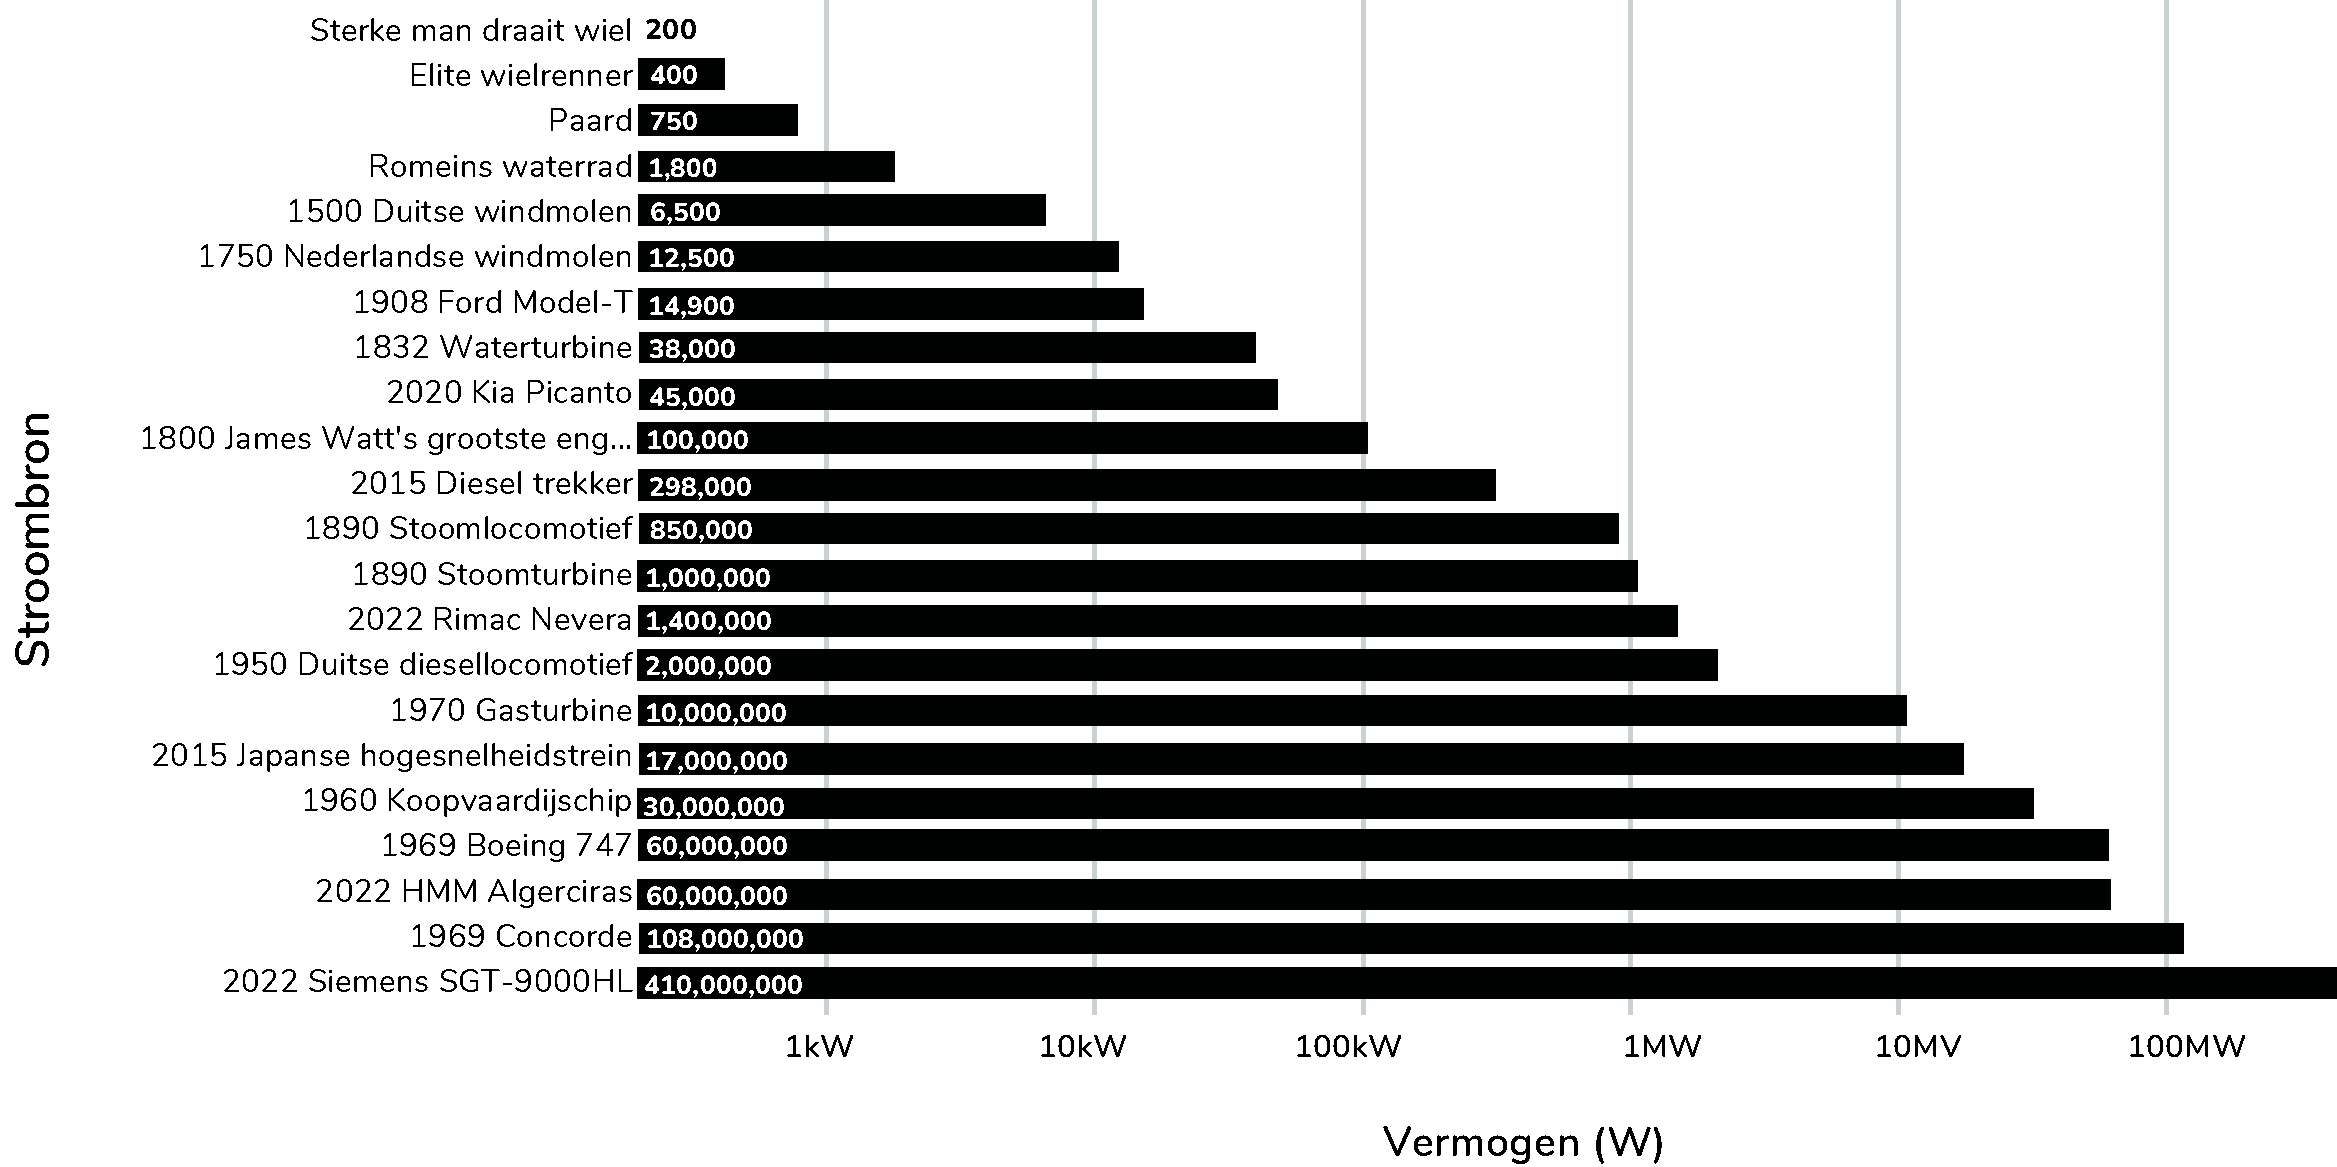
\includegraphics[width=\textwidth]{figures/fig9.pdf}
    \caption[Maximale energieproductie gedurende de afgelopen 3.000 jaar]{Maximale energieproductie gedurende de afgelopen 3.000 jaar}
    \label{fig9}
\end{figure}

Een paard kan ongeveer 750 watt aan vermogen produceren, en een topwielrenner kan ongeveer 400 watt produceren gedurende ongeveer een uur. De Ford Model-T produceerde op volle snelheid 14,9 kW in 1908. Een moderne compacte auto zoals de Kia Picanto produceert ongeveer 45 kW. De krachtigste sportwagen ter wereld, de Rimac Nevera, produceert meer dan 1,4 MW aan vermogen. Rond 1890 draaide een grote stoomlocomotief op volle snelheid 850 kW. In 1950 leverde een krachtige Duitse diesellocomotief 2MW, en in 2015 leverde een snelle Japanse trein 17 MW. In 1960 draaide een Japanse diesel aangedreven koopvaardijschip op 30 MW, terwijl in 1969 een Boeing 747 op 60 MW draaide, en de vier motoren van de supersonische Concorde 108 MW zouden produceren bij een kruissnelheid van 2.400 km/u. De motor van de HMM Algeciras levert 60 MW. Van het paard tot de HMM Algeciras en Boeing 747 heeft de mensheid een 80.000-voudige toename in het vermogen voor vervoer gezien.

Smil vergelijkt ook het maximale vermogen op het land door de tijd. Terwijl een boer die een koolveld schoffelde 50W zou produceren, zou een boer die met twee kleine paarden ploegde 1.000 W tot zijn beschikking hebben. Met een kleine tractor kon een boer in 1950 oogsten met 50 kW aan vermogen tot zijn beschikking. En in 2015 kon een boer met een grote dieseltrekker beschikken over 298 kW aan vermogen. In drie eeuwen van technologische vooruitgang is het vermogen dat een boer tot zijn beschikking heeft, 6.000 keer zo groot geworden.

Voordat koolwaterstoffen bestonden, kon de mensheid slechts beperkte hoeveelheden bruikbare energie gebruiken, en alleen in de buurt van waterraderen en windmolens. Met koolwaterstoffen kunnen op elk moment en overal grote hoeveelheden energie worden opgewekt. Dit maakt het mogelijk om groeiende bevolkingscentra te ondersteunen, handel tussen deze bevolkingscentra te vergroten en de arbeidsproductiviteit te verhogen.

Alex Epstein brengt een overtuigend argument voor hoe koolwaterstofbrandstoffen de basis vormen voor moderne welvaart.\autocite{97} Tot de zestiende eeuw was het leven overal voornamelijk afhankelijk van het verbranden van hout voor de energievoorziening. In vergelijking met moderne koolwaterstoffen bevat hout veel minder energie per eenheid gewicht. Nadat het gebruik van steenkool in de zestiende eeuw startte, gevolgd door olie\index{olie} en gas, nam de hoeveelheid beschikbare energie per persoon enorm toe, en daarmee ook onze levenskwaliteit. Om het echte voordeel van energie voor ons leven te visualiseren, nodigt Epstein ons uit om de energie die we vandaag verbruiken te zien in het licht van het energieverbruik van mensen die taken voor ons uitvoeren. Volgens die maatstaf vindt hij dat de gemiddelde Amerikaan dagelijks over 186.000 calorieën beschikt, of het energie-equivalent van 93 mensen. Vóór moderne brandstoffen was deze hoeveelheid energie zelden voor iemand beschikbaar. Alleen de rijkste koningen konden dromen van het hebben van zoveel energie tot hun dagelijkse beschikking, hetzij in de vorm van brandbaar hout hetzij van tot slaaf gemaakte mensen.

\begin{figure}[!htb]
\centering
    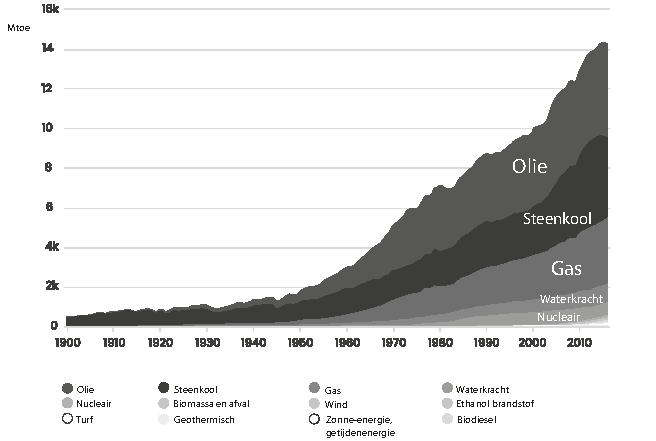
\includegraphics[width=\textwidth]{figures/fig10.pdf}
\caption[Wereldwijd primair energieverbruik]{Wereldwijd primair energieverbruik\footnotemark}
\label{fig10}
\end{figure}
\autocite{98}

\begin{figure}[!htb]
\centering
    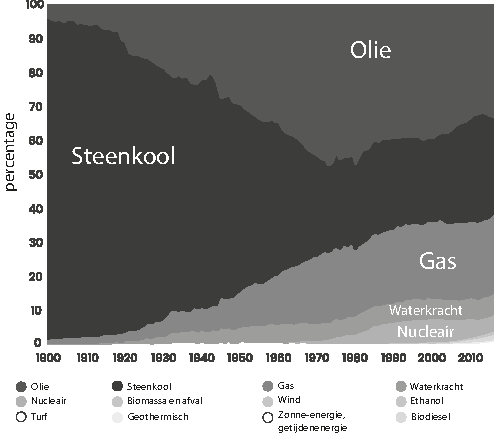
\includegraphics[width=\textwidth]{figures/fig11.pdf}
\caption[Wereldwijd primair energieverbruik, procentueel]{Wereldwijd primair energieverbruik, procentueel\footnotemark}
\label{fig11}
\end{figure}
\autocite{99}

De Industriële Revolutie, die wereldwijd de levensstandaard transformeerde, was onlosmakelijk verbonden met de uitvinding van de stoommachine en het massale gebruik van kolen om de productiviteit van werknemers te verhogen. Tot het begin van de twintigste eeuw was steenkool de belangrijkste energiebron. De uitvinding van de interne verbrandingsmotor maakte een massaal gebruik van olie\index{olie} mogelijk, die per gewichtseenheid meer energie levert en daarom efficiënter te vervoeren en in transport te gebruiken is. De twintigste eeuw zag een snelle stijging van het wereldwijde gebruik van olie\index{olie}, en in de tweede helft van de twintigste eeuw groeide het gebruik van gas het snelst. Tegenwoordig is ongeveer 80\% van het wereldwijde energieverbruik afkomstig van deze drie koolwaterstofbrandstoffen.

Naarmate technologie verbetert en de levensstandaard stijgt, verwachtten we meer verschuiving naar natuurlijk gas voor energieopwekking, omdat het de minste vervuiling veroorzaakt van alle koolwaterstofbrandstoffen. Desondanks zal er realistisch gezien nog steeds een enorme vraag zijn naar vermogen uit steenkool. Dit komt doordat de enige praktische alternatieven voor veel mensen over de hele wereld laag energetische bronnen zijn, die onbetrouwbaar en niet continu beschikbaar zijn. Steenkool is goedkoop en de technologieën die worden gebruikt om er energie uit op te wekken zijn al decennia lang geperfectioneerd. Moderne schone steenkooltechnologie verlaagt de hoeveelheid schadelijke emissies die door het verbruik ervan wordt veroorzaakt drastisch. De voordelen van betrouwbare energie zijn aanvaardbaar gebleken voor de overgrote meerderheid van mensen die zich verplaatsen naar gebieden met steenkoolcentrales en betrouwbare energie, en weg van gebieden zonder steenkoolcentrales en betrouwbare energie.

In 1802 bouwde Richard Trevithick de eerste werkende spoorweg-stoom\-loco\-motief. Deze gebruikte kolen om treinwagons te laten rijden. Rond dezelfde tijd werd de stoomboot uitgevonden. Die werkte volgens hetzelfde principe. In 1885 werd de auto uitgevonden en in 1902 het vliegtuig. Deze technologieën hebben gedurende meer dan twee eeuwen de kosten van transport verlaagd en de beschikbaarheid ervan verhoogd. Het vervoer van goederen kost vandaag de dag nog maar een fractie van wat het vroeger kostte vóór de komst van koolwaterstofenergie. Hierdoor is onze handelscapaciteit aanzienlijk gegroeid. Ook is de wereldwijde arbeidsdeling\index{arbeidsdeling} enorm toegenomen, wat de menselijke productiviteit verder heeft verhoogd.

Het moderne kapitalisme\index{kapitalisme} en de wereldwijde arbeidsdeling\index{arbeidsdeling} die in de negentiende eeuw ontstonden, zouden simpelweg onmogelijk zijn geweest zonder het gebruik van energiebronnen die zijn gebaseerd op koolwaterstoffen. Deze energiebronnen verhoogden de arbeidsproductiviteit en levensstandaard aanzienlijk. Zonder deze energiebronnen om moderne motoren en machines van brandstof te voorzien, zou de arbeidsproductiviteit niet zijn gestegen tot het punt waarop arbeiders veel meer waarde konden produceren dan ze nodig hadden om te overleven. Hierdoor hadden ze een aanzienlijk aantal middelen om met anderen te verhandelen. De accumulatie van kapitaal\index{kapitaal} nam op een fundamenteel andere manier toe nadat deze brandstoffen het voor mensen mogelijk maakten om snel groeiende hoeveelheden energie te gebruiken.

Het contrast tussen verschillende plekken op de wereld, en de veranderingen door de geschiedenis heen, illustreren hoe enorm waardevol toegang tot grote hoeveelheden vermogen is. Onze moderne wereld is grotendeels het product van de ontwikkeling van technologieën die ons regelmatig toegang geven tot toenemende hoeveelheden energie. Moderne beschaving\index{beschaving} en de meeste van haar prestaties zouden niet mogelijk zijn zonder niveaus van energieverbruik die volledig afwijkend zijn van de historische gegevens.

\begin{figure}[!htb]
\centering
    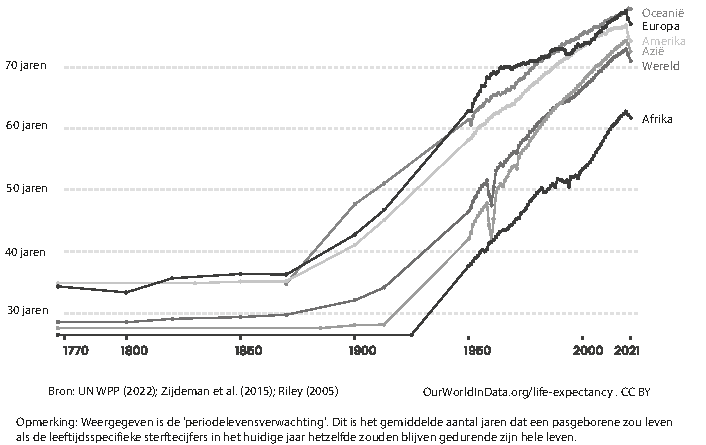
\includegraphics[width=\textwidth]{figures/fig12.pdf}
    \caption[Wereldwijde levensverwachting, 1770-2021]{Wereldwijde levensverwachting, 1770-2021.}
    \label{fig12}
\end{figure}

Gegevens uit 118 landen met bevolkingen groter dan vier miljoen in 2005 laten de correlatie zien tussen energieconsumptie per persoon en verbeterde toegang tot water, levensverwachting, kindersterfte, gemiddeld aantal schooljaren, elektrificatie en bruto nationaal inkomen. \autocite{100} De relaties zijn zeer duidelijk: hoe meer een samenleving in staat is energie te benutten en te verbruiken, hoe beter het in staat is om te voorzien in de basisbehoeften van het moderne leven.

Als we beter naar het bbp kijken, is de relatie zeer duidelijk en al heel lang aanwezig: een groter energieverbruik heeft een sterke correlatie met grotere economische productie\index{productie}, en daardoor een hogere levensstandaard, zoals duidelijk is te zien in Figuur 13.

\begin{figure}[H]
\centering
    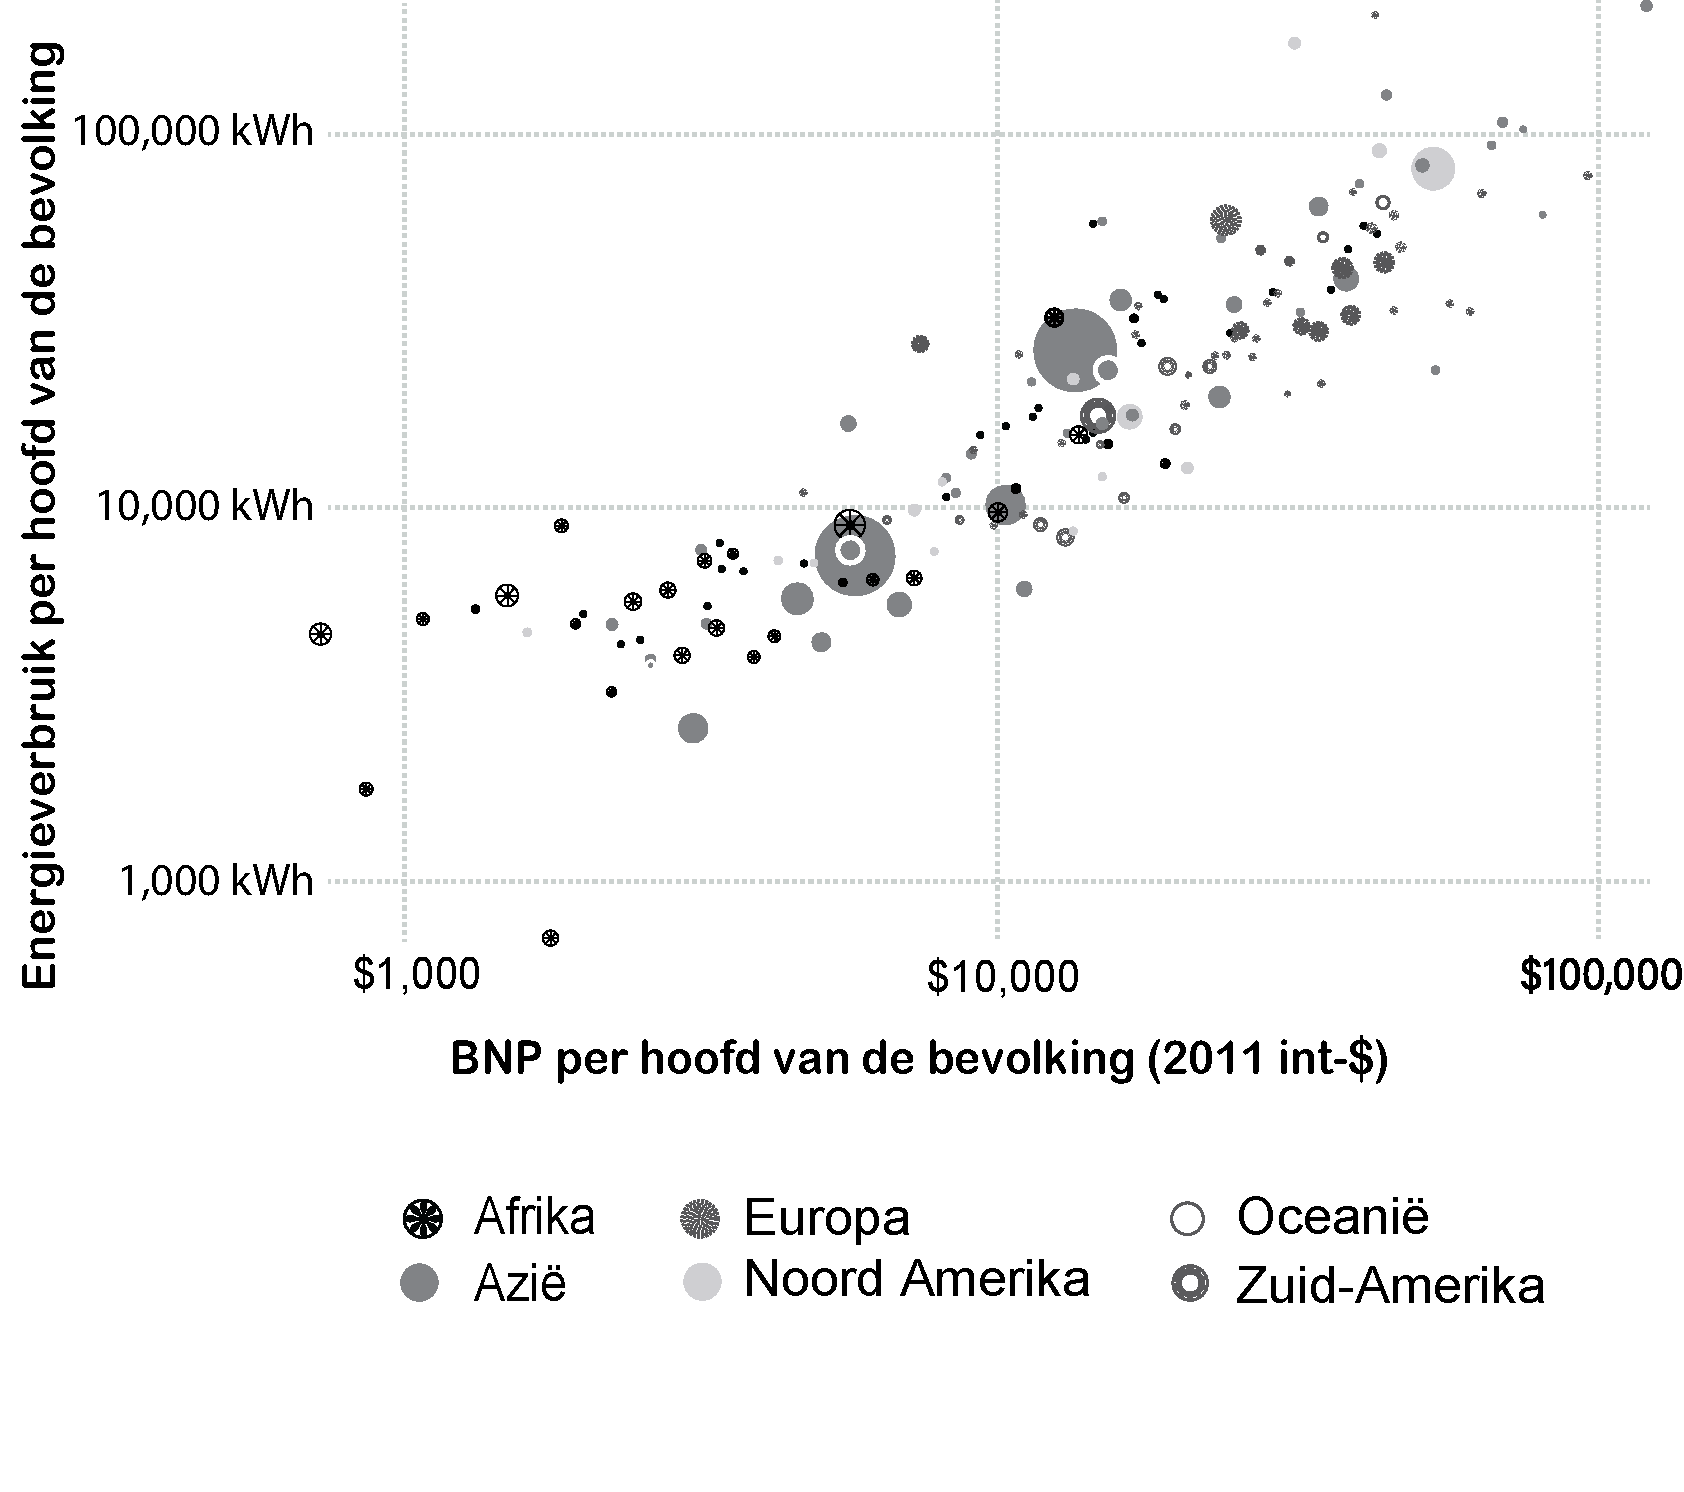
\includegraphics[height=8cm]{figures/fig13.pdf}
    \caption[Energieverbruik per persoon versus bnp, 2015]{Energieverbruik per persoon versus bnp, 2015\footnotemark}
    \label{fig12}
\end{figure}
\autocite{101}

\begin{figure}[H]
\centering
    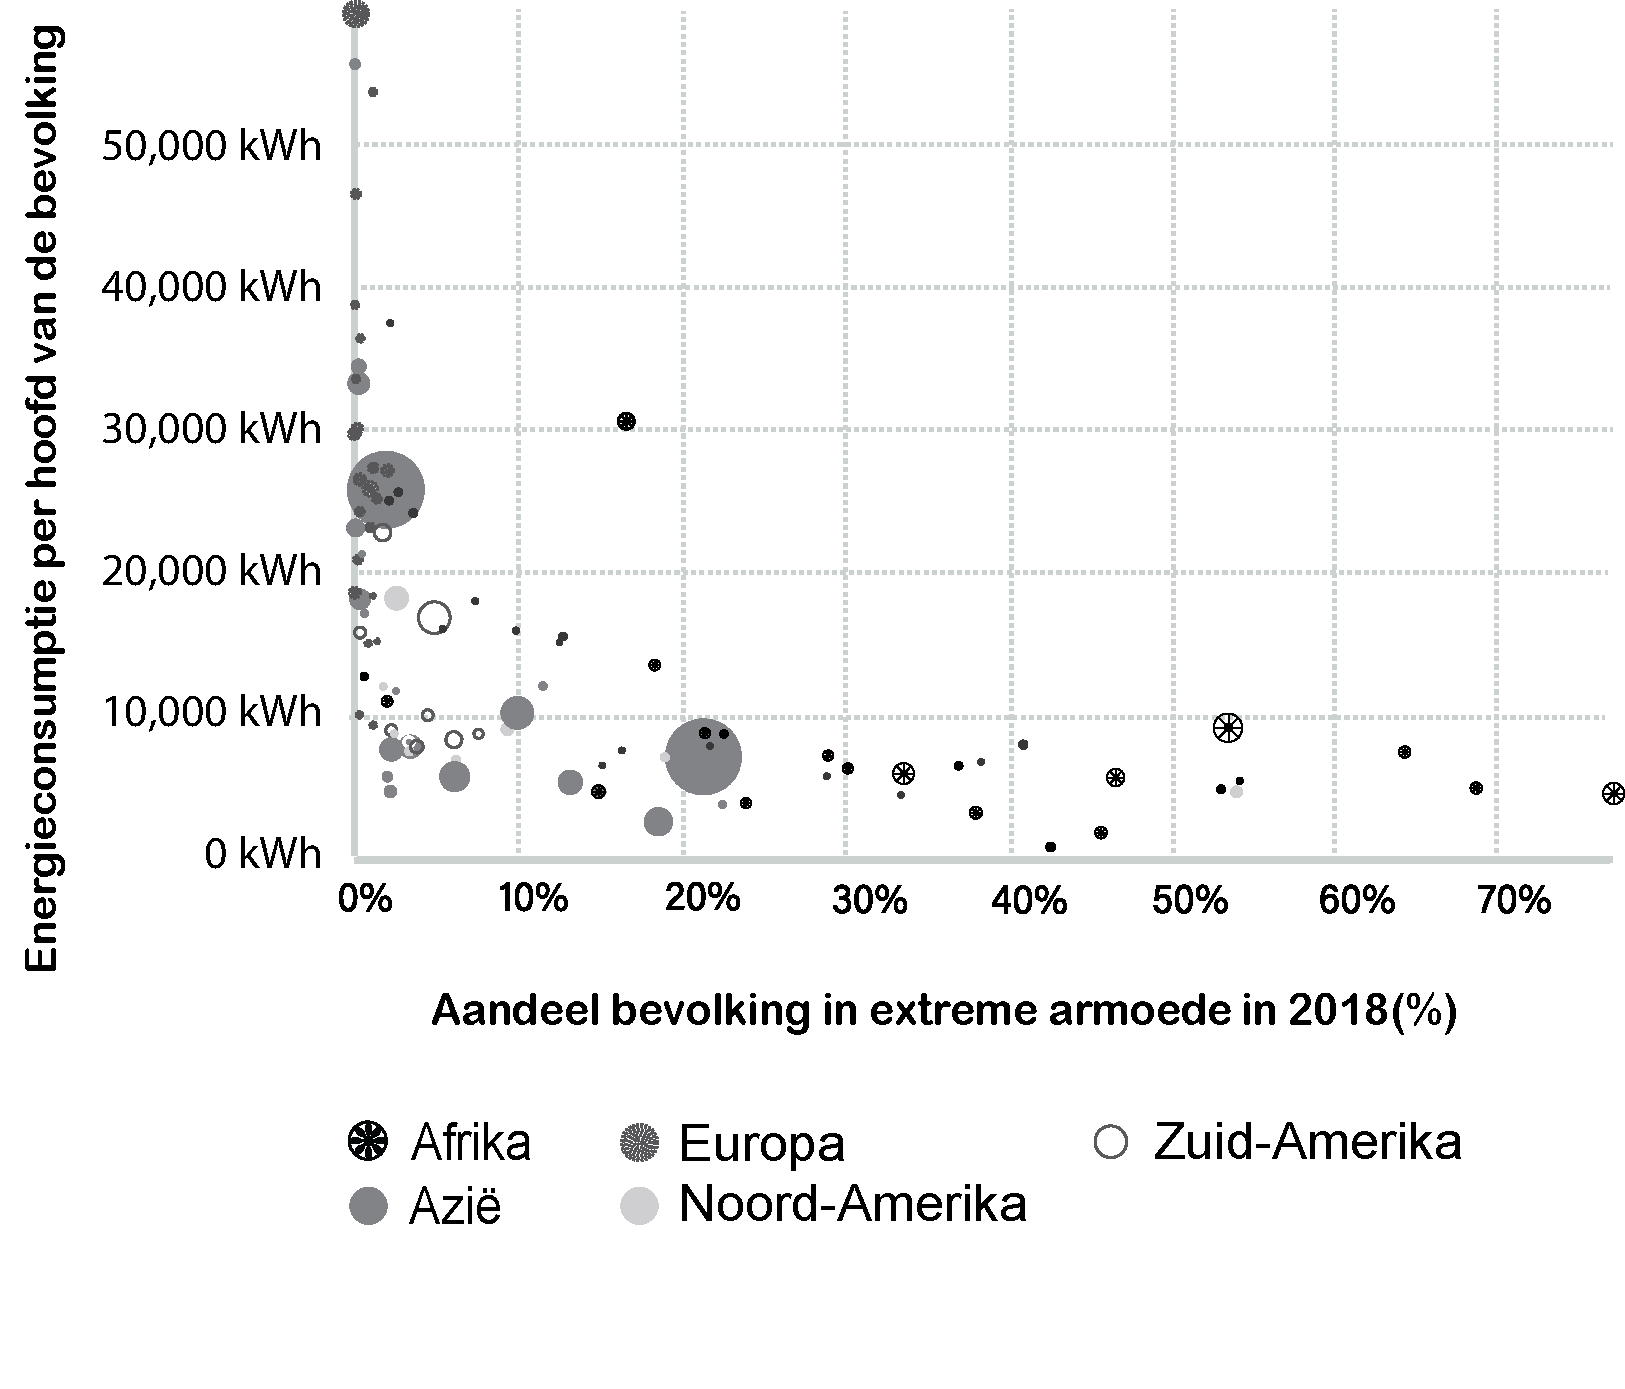
\includegraphics[height=8cm]{figures/fig14.pdf}
    \caption[Energieverbruik per persoon versus percentage van de bevolking in extreme armoede]{Energieverbruik per persoon versus percentage van de bevolking in extreme armoede\footnotemark}
    \label{fig12}
\end{figure}
\autocite{102}

Figuur 14 toont de relatie tussen het energieverbruik per persoon en het deel van de bevolking dat in extreme armoede leeft. Geen enkel land dat extreme armoede heeft uitgeroeid, verbruikt minder dan 10.000 kWh per hoofd van de bevolking per jaar. En geen enkel land waarin meer dan 20\% van de bevolking in extreme armoede leeft, verbruikt meer dan 10.000 kWh per hoofd van de bevolking per jaar.

De vooruitgang van de mensheid is aangedreven door technologische ontwikkelingen die de energie opgeslagen in koolwaterstofbrandstoffen vrijmaken. Het feit dat de meeste mensen vandaag de dag beschermd leven tegen de meeste gevaren van de natuur, warm kunnen blijven in de winter, en sneller kunnen reizen dan als ze zouden lopen, is het resultaat van innovaties tijdens de Industriële Revolutie. Deze gaven ons diverse soorten motoren om toegang te krijgen tot de energie in de drie belangrijkste koolwaterstofbrandstoffen: steenkool, olie\index{olie}, en gas. Zoals Philip Cross het verwoordde:

\begin{blockquotebox}
    De geschiedenis van economische ontwikkeling is de geschiedenis van de hoeveelheid energie die onder menselijke controle is gebracht. Economische historici hebben de nauwe relatie opgemerkt tussen economische groei en energieverbruik naarmate we meer energie voor ons aan het werk zetten. De Amerikaanse econoom Deirdre McCloskey noemde de toename van het energieverbruik dat rond 1800 begon ``de Grote Verrijking'', beter bekend als \textit{The Great Enrichment}. De voordelen voor de mensheid zijn enorm geweest, de levensverwachting is verlengd, de voedselproductie is verhoogd om de groeiende bevolking te ondersteunen, en de levensstandaard voor de meeste mensen is verhoogd tot niveaus waar zelfs leden van het koningshuis een paar eeuwen geleden niet van konden dromen.
    \par\vspace{1em}\noindent
    De overleden Italiaanse economiehistoricus Carlo Cipolla schreef zowel de Agrarische Revolutie duizenden jaren geleden als de Industriële Revolutie, die aan het einde van de achttiende eeuw begon, toe aan de hoeveelheid energie die werd gebruikt. In de Agrarische Revolutie gingen mensen over van jagen en verzamelen naar het cultiveren en temmen van de energie in planten en dieren, ook al zijn meeste planten en dieren geen erg efficiënte omzetters van energie. Vuur, wind en water verhoogden ook de energie die mensen tot hun beschikking hadden. Na verloop van tijd werden mensen efficiënter in het gebruik van al deze energiebronnen, door middel van rudimentaire landbouwwerktuigen, irrigatie, open haarden, watermolens en zeilboten.
    \par\vspace{1em}\noindent
    Fossiele brandstoffen speelden een verwaarloosbare rol in de energievoorziening tot de Industriële Revolutie. Hoewel alles op de planeet een mogelijke energiebron is, bleken fossiele brandstoffen bijzonder efficiënt en handig om te voldoen aan de energie-eisen van industrialisatie. In de woorden van Cipolla kan de Industriële Revolutie worden beschouwd als ``het proces waarbij de grootschalige exploitatie van nieuwe energiebronnen door middel van anorganische omzetters in gang werd gezet''. Steenkool was de eerste wijdverbreide bron van anorganische energie. Het aandeel ervan steeg van 10 procent van de energievoorziening in Groot-Brittannië in 1560 tot 60 procent in 1750. Dit resulteerde in het beëindigen van de ontbossing van Groot-Brittannië. Dit startte een cumulatief proces, waarbij een groeiende energievoorziening meer economische groei aanwakkerde. Dit stimuleerde op zijn beurt het onderwijs\index{onderwijs}, wat leidde tot de ontdekking van nieuwe energiebronnen, met name andere fossiele brandstoffen.
    \par\vspace{1em}\noindent
    De eerste commerciële toepassing van koolwaterstofbrandstoffen was kerosine om licht te maken en zo een einde te maken aan onze eeuwig terugkerende val in duisternis na zonsondergang. (Dit stopte de grootschalige jacht op walvissen, waarvan de olie\index{olie} tot dan toe de voornaamste bron van binnenverlichting was.) De VS liepen voorop in de exploitatie van olie\index{olie} in de 19e eeuw, een rol die ze vandaag de dag opnieuw op zich neemt dankzij innovatieve technologieën voor de ontwikkeling van schalie-afzettingen. 1860 is het olietijdperk door de ontwikkeling van boortechnologie in Pennsylvania echt van start gegaan.\footnotemark
\end{blockquotebox}
\autocite{103}

Terwijl mensen nieuwe technologieën blijven ontdekken om energie te gebruiken voor onze doeleinden, verlagen we de reële energiekosten. Fouquet schat in een studie naar de energieprijzen in het Verenigd Koninkrijk tussen 1300 en 2000 dat de verwarmingskosten met meer dan 80\% zijn gedaald. De kosten van energie zijn gedaald met 94\%, die van  vrachtvervoer met 95\%, van passagiersvervoer met 91\% en de kosten voor verlichting zijn gedaald met 99,98\%. Deze dalingen worden geïllustreerd in Figuren 15 en 16.\autocite{104}

\begin{figure}[!htb]
\centering
    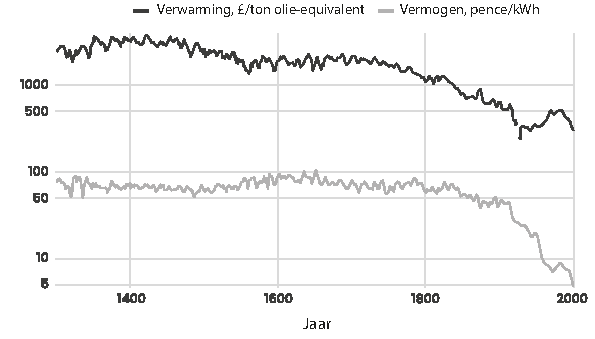
\includegraphics[width=\textwidth]{figures/fig15.pdf}
    \caption[Kosten van verwarming en energie in het Verenigd Koninkrijk, 1300-2000.]{Kosten van verwarming en energie in het Verenigd Koninkrijk, 1300-2000}
    \label{fig15}
\end{figure}

\begin{figure}[!htb]
\centering
    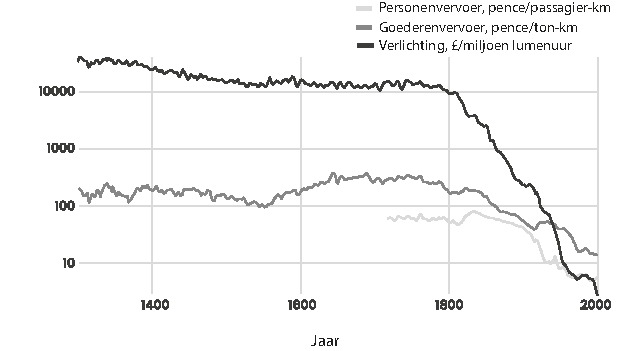
\includegraphics[width=\textwidth]{figures/fig16.pdf}
    \caption[Kosten van verlichting en transport in het Verenigd Koninkrijk, 1300-2000]{Kosten van verlichting en transport in het Verenigd Koninkrijk, 1300-2000}
    \label{fig16}
\end{figure}


\hypertarget{alternatieven-voor-vermogen-uit-koolwaterstof}{%
\section{Alternatieven voor vermogen uit koolwaterstof}\label{alternatieven-voor-vermogen-uit-koolwaterstof}}

Ondanks de verbazingwekkende en onmiskenbare voordelen die hoogwaardige koolwaterstoffen onze wereld hebben gebracht, gelooft een meerderheid van de economen en het publiek dat deze vervangen moeten en zullen worden door alternatieve energiebronnen. Deze afkeer ontstond initieel op basis van de prijsstijgingen van koolwaterstofbrandstoffen in de jaren `70, veroorzaakt door inflatoir monetair beleid, en maakte doemdenkers populair die voorspelden dat we op het punt stonden om deze enorm overvloedige brandstoffen uit te putten. Toen de productie\index{productie} decennia lang bleef toenemen en bewezen reserves\index{reserves} zelfs nog meer groeiden, is deze specifieke hysterie afgenomen. Maar de anti-koolwaterstofhysterie heeft een nieuwe reden gevonden. Onduidelijk en ontoetsbaar pseudowetenschappelijk bijgeloof over broeikasgasemissies als de regelknop voor het weer op aarde zijn nu de reden waarom we van koolwaterstoffen af moeten en over moeten stappen naar ``duurzame''  alternatieven, zoals wind, zon en biobrandstoffen. Ik betoog dat de vijandigheid van de moderne door de overheid\index{overheid} gefinancierde wetenschap tegenover koolwaterstofbrandstoffen zijn wortels heeft in het inflatoire monetaire beleid. Dit beleid verhoogt niet alleen de prijzen van deze essentiële brandstoffen, maar stelt de overheid\index{overheid} ook in staat om de wetenschap te financieren en te dicteren. De overheid\index{overheid} wil brandstofvrije alternatieven promoten, omdat deze minder gevoelig zijn voor monetaire inflatie\index{inflatie} dan energierijke brandstoffen die op de wereldmarkt worden geproduceerd.

Promotors van wind- en zonne-energie beweren vaak dat deze energiebronnen goedkoper zijn dan koolwaterstoffen, omdat hun ``brandstof''  gratis is -- er zijn immers geen kosten verbonden aan zonlicht en wind. Maar dit is een goed voorbeeld van een gebrekkig economisch\index{economisch} redeneren, omdat het geen marginale beslissingen analyseert. Marginale analyse kan ons helpen het onoplosbare probleem met wind- en zonne-energie als alternatieven voor koolwaterstoffen te begrijpen. Energie wordt niet als geheel of abstract gekocht; het wordt aan de marge gekocht, in specifieke hoeveelheden, met bepaalde intensiteiten, voor een bepaalde tijd. Energie zelf is niet het economische goed, maar vermogen is dat wel. De geavanceerde machines die onze moderne beschaving\index{beschaving} mogelijk maken, hebben stroom nodig die op aanvraag en in specifieke, gecontroleerde intensiteiten geleverd kan worden. De stroom die windmolens en zonnepanelen leveren is echter onvoorspelbaar en komt in vlagen, aangezien deze energie alleen beschikbaar is wanneer de wind waait of de zon schijnt. In tegenstelling hiertoe zijn koolwaterstofenergiebronnen gemakkelijk vervoerbaar en op te slaan, wat betekent dat ze in grote hoeveelheden aanwezig kunnen zijn wanneer en waar ze nodig zijn. Zodra moderne machines en infrastructuur eenmaal zijn gebouwd, kan koolwaterstofenergie op aanvraag en op de precieze intensiteit die nodig is beschikbaar worden gesteld tegen zeer lage marginale kosten.

Of het nu gaat om het elektriciteitsnet, ziekenhuizen, couveuses, koelkasten, verwarming en koeling, internetservers, talloze online diensten, luchthavens of talloze vormen van moderne infrastructuur; de moderne beschaving\index{beschaving} heeft haar machines nodig om continu te werken, ongeacht de weersomstandigheden. Geen enkel modern bedrijf\index{bedrijf} kan zijn fabrieken, servers of kantoren laten draaien volgens de grillen van het weer. Om hoogproductieve apparatuur te laten functioneren, is een lage marginale energiekost niet alleen nodig, maar ook op elk moment vereist. Hoewel de marginale kosten van hernieuwbare energiebrandstoffen inderdaad gratis zijn als de zon schijnt en de wind waait, zijn ze oneindig als dit niet het geval is. Geen enkele kapitaalinvestering zal de zon eeuwig laten schijnen en de wind altijd laten waaien wanneer een machine energie nodig heeft. Wanneer de zon niet schijnt, zijn de marginale kosten van zonne-energie oneindig, en wanneer de wind niet waait, zijn de marginale kosten van windenergie oneindig. Als wind- en zonne-energie inderdaad als alternatief voor koolwaterstoffen werden gebruikt, zou een moderne industriële samenleving niet langer mogelijk zijn.

Door overheidsbeleid dat zwaar inzet op subsidies, is het gebruik van wind- en zonne-energie toegenomen. Deze afhankelijkheid heeft echter catastrofale gevolgen. Het verlaagt de voorspelbare piekbelasting voor elk individueel nutsbedrijf, aangezien de piekvraag nu kan optreden op een moment dat sommige brandstoffen niet beschikbaar zijn. Voor de volledige capaciteit van de piekbelasting moet men dan ook volledig vertrouwen op koolwaterstoffen. Hierdoor worden investeringen in kostbare wind- en zonne-infrastructuur praktisch overbodig. Hoewel het inderdaad het verbruik van koolwaterstofbrandstoffen kan verminderen, maken de wisselvalligheid en onvoorspelbaarheid van wind- en zonne-energie het beheer en onderhoud van de koolwaterstofcentrales en netwerken duurder en heffen dus grotendeels de gemaakte besparingen op. Om deze reden bestaat stroomopwekking uit wind en zon slechts in de mate waarin het gesubsidieerd is door overheidsuitgaven.

Mensen streven als ze economisch\index{economisch} handelen voortdurend naar manieren om hun productiviteit te verhogen. In de context van energie is dit altijd in de vorm van het verhogen van de energiedichtheid van de krachtbronnen die we gebruiken om aan onze behoeften te voldoen, gemeten in MJ/kg. Om zonne- en windenergie geschikt te maken voor het moderne leven, zou er gebruik moeten worden gemaakt van batterijen. Deze technologie heeft echter een enorm lage energie per gewicht, rond de 0,5 MJ/kg. Dit is ruwweg 1\% van de energiedichtheid van olie\index{olie} of aardgas. Batterijen zijn ook erg duur, en daarom worden ze voornamelijk gebruikt in gebieden waar motoren niet praktisch zijn.

\vspace{-1em}
\hypertarget{energie-en-vrijheid}{%
\section{Energie en vrijheid}\label{energie-en-vrijheid}}

Toen de menselijke productiviteit erg laag was en de technologie primitief, waren er weinig manieren voor mensen om werk te verzetten om in hun behoeften te voorzien, afgezien van hun eigen arbeid. Een van de meest effectieve energiebronnen was de arbeid van andere mensen. Als een mens echter een zeer lage productiviteit had, had hij zijn eigen arbeid nodig om te overleven. Dit betekende dat hij zelden in staat was om anderen te betalen om voor hem te werken, en anderen konden hem zelden betalen. Kansen voor wederzijds voordelige arbeid zouden schaars zijn in zo\textquotesingle n situatie. Als een man de energie van een ander wilde verwerven om in zijn eigen behoeften te voorzien, zou hij waarschijnlijk de ander moeten dwingen om zijn energie te leveren ten koste van zijn eigen behoeften. Slavernij was in een wereld met primitieve energiebronnen een veel voorkomend instituut, omdat het beschikken over de energie van een ander mens bijna een verdubbeling van de totale hoeveelheid beschikbare energie om in je behoeften te voorzien betekende. Lage productiviteit maakt overleven een lijdensweg, en de arbeid van anderen wordt enorm waardevol, wat slavernij winstgevend maakt.

Naarmate de productiviteit toeneemt door de ontwikkeling van technologie en het gebruik van niet-menselijke energiebronnen, wordt het mogelijk voor mensen om in hun behoeften te voorzien door de inzet van toenemende hoeveelheden energie-intensief kapitaal\index{kapitaal} in plaats van de slavenarbeid van anderen. De dringende behoefte aan arbeid van anderen die aanzet hen tot slaaf te maken, neemt af.

Machines kunnen veel van het werk van de slaaf doen en ze veroorzaken minder problemen dan een mens met een constante drang om vrij te zijn. Omdat machines de productiviteit van een werknemer verhogen, is het mogelijk voor hem om aan zijn eigen behoeften en die van een werkgever die het kapitaal\index{kapitaal} levert, te voldoen. Naarmate de machines duurder en een integraler onderdeel van het economisch\index{economisch} productieproces\index{productieproces} worden, neemt het belang en de verantwoordelijkheid van de werknemer toe en wordt slavernij een volstrekt ongeschikte manier om het werk gedaan te krijgen. Slaven die taken met hoge productiviteit moeten uitvoeren en dure machines gebruiken, zijn waarschijnlijk niet gemotiveerd om deze productief in te zetten, en ze kunnen zeer waarschijnlijk sabotage plegen. Naarmate machines en energie de productiviteit van arbeid verhoogden, nam de kans toe dat werknemers op vrijwillige basis in plaats van onder dwang werden ingeschakeld.

In de context van energiearmoede was het erg belangrijk om de beschikking over de energie van een ander mens te krijgen. Maar in de huidige context van energieovervloed, waar een persoon in een rijk, geïndustrialiseerd ontwikkeld land dagelijks de energie van 100 mensen gebruikt, draagt het toevoegen van een extra mens als slaaf weinig marginaal vermogen bij. Naarmate energiebronnen het menselijk leven binnendrongen, verbeterde onze productiviteit en levensstandaard, waardoor het marginale voordeel van het tot slaaf maken van een mens aanzienlijk kromp. Bovendien, naarmate kapitaalopbouw en moderne machines centraler kwamen te staan binnen het productieproces\index{productieproces}, werd de capaciteit van de arbeider om de machines te onderhouden en niet te beschadigen veel waardevoller dan de kracht die zijn handen boden. De inzet van een slaaf voor zijn meester was niet langer waardevol wanneer een machine veel meer goedkopere energie kon leveren voor zwaar werk. De intelligentie en integriteit van werknemers bij het beheer en onderhoud van machines werd veel waardevoller dan hun brute kracht. Het is geen toeval dat de afschaffing van slavernij zich verspreidde met de industrialisatie. Groot-Brittannië leidde de wereld in het afschaffen van de slavernij, juist omdat het wereldwijd met industrialisatie voorop liep. Waar de stoommachine en de elektrische generator kwamen, verdween de slavernij snel. Slavernij bestaat tegenwoordig nog steeds, maar alleen in industrieel primitieve samenlevingen met weinig kapitaalopbouw en energiegebruik. De economie van machines maakt slavernij economisch\index{economisch} veel minder praktisch. Het maakt zwaar werk, dat door slavernij werd geleverd, voor een zeer lage kostprijs beschikbaar, en verhoogt de productiviteit en waarde van de arbeidstijd van een werknemer tot een punt waarop zijn vrijwillige samenwerking waardevoller is dan elke slavenarbeid die hij zou kunnen uitvoeren.

Hoogwaardige machines zijn ook een ondergewaardeerde aanjager van de emancipatie van vrouwen. In een primitieve economie met weinig krachtige machines was menselijke kracht uiterst waardevol, en de sterkste mensen waren het meest productief. Mannen zijn vanwege een groter lichaam met meer spiermassa gemiddeld sterker dan vrouwen en waren daarom waardevoller in arbeid en vrouwen waren afhankelijk van mannen om te overleven. Toen moderne energie-intensieve machines de meeste fysieke taken overnamen, zoals vervoeren, tillen, pompen, ploegen, en beschermen tegen de natuur en dieren, verminderde het belang van fysieke kracht in vergelijking tot de behoefte aan cognitieve kracht. Hierdoor werd het voordeel dat mannen dankzij hun kracht hadden ten opzichte van vrouwen, verminderd. In een moderne, energierijke economie vereisen de meest productieve en best beloonde banen geen fysieke kracht meer. De sterkste en machtigste mensen in de samenleving zijn niet langer degenen die de meeste hulpbronnen kunnen veiligstellen. Machines doen het zwaarste werk en de hoogste beloningen gaan naar degenen met cognitieve vaardigheden om deze machines te beheren. Vrouwen kunnen in een industriële en informatie-economie veel gemakkelijker onafhankelijk voor hun eigen onderhoud zorgen dan in een primitieve economie. Het is geen toeval dat de emancipatie van vrouwen samengaat met industrialisatie. De rijkste en meest geïndustrialiseerde samenlevingen hebben de best presterende en meest onafhankelijke vrouwen, terwijl in pre-industriële samenlevingen de onderdrukking van vrouwen nog steeds veel voorkomt.
